\subsection*{Ausblick: Matrizen in der künstlichen Intelligenz}

% Wir interpretieren Matrizen in diesem Kurs als geometrische Abbildungen. Das hilft uns dabei, Aussagen über Matrizen zu verstehen, die ohne diese Interpretation sehr abstrakt wären. Matrizen sind aber auch ausserhalb der Geometrie von grosser Bedeutung. Zum Beispiel in der Informatik.

Viele komplexe Probleme lassen sich mit Computern effizient lösen. Dabei werden die Computer so programmiert, dass sie eine Reihe von Anweisungen durchführen – einen Algorithmus – und so die gewünschte Lösung liefern.

Es gibt aber Fragestellungen, bei denen diese klassischen Vorgehensweise versagt. Das ist zum Beispiel dann der Fall, wenn man bestimmte Informationen richtig interpretieren soll. Ein typischen Beispiel dafür ist die Erkennung von Handschriften. 

\begin{center}
    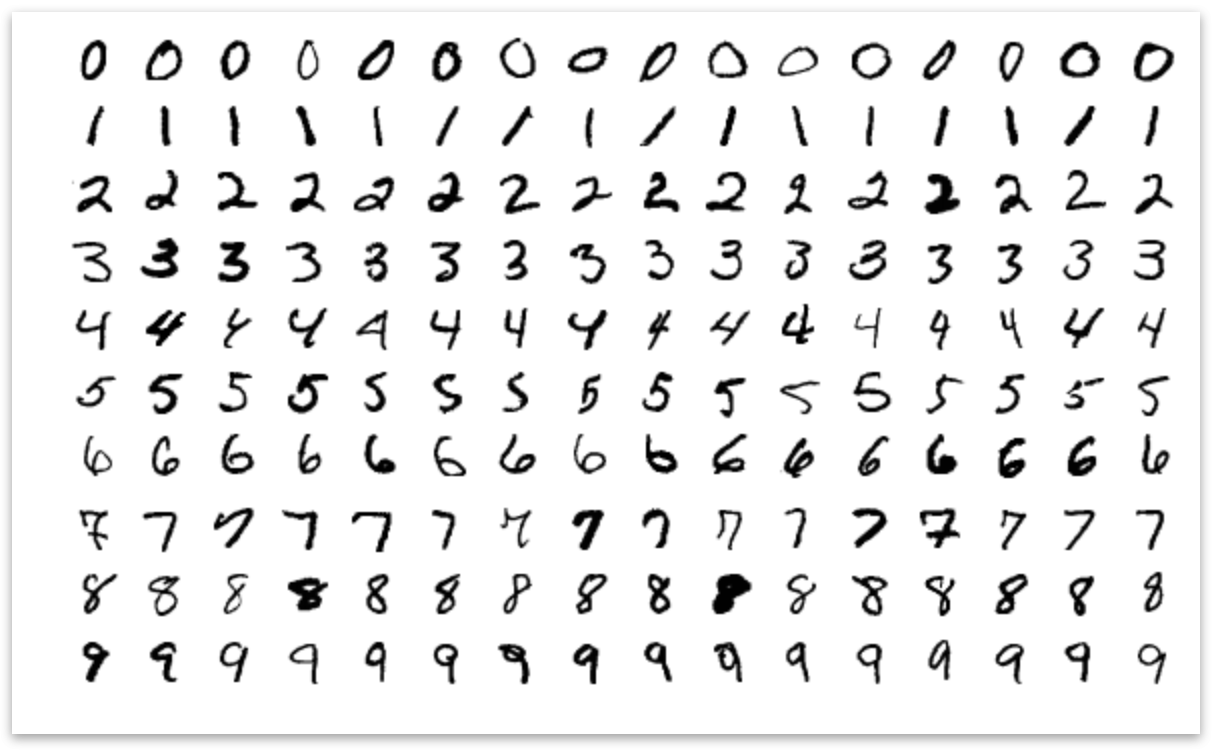
\includegraphics[width = 0.5 \textwidth]{media/ziffern.png}
\end{center}

Während wir problemlos die Ziffern oben erkennen können, ist das für einen Computer keinesfalls einfach, weil die gleiche Ziffer ganz unterschiedlich dargestellt werden kann. 
Für solche Probleme hat man grosse Erfolge durch den Einsatz von maschinellem Lernen erzielt. Dabei wird ein Programm zuerst trainiert, damit es die richtigen Muster erlernt.

Es gibt verschiedene Arten von lernenden Systemen. Für die Erkennung der Handschrift eignet sich ein sogenanntes neuronales Netz.
Etwas vereinfacht wird dabei ein grosser Vektor mit einer grossen Matrix multipliziert. Für     die Erkennung der Ziffern muss man sich das wie folgt vorstellen.
%Dabei wird das Programm zuerst «trainiert», damit der Computer die richtigen Muster «erlernt». Im Grunde geht das wie folgt:

\begin{center}
    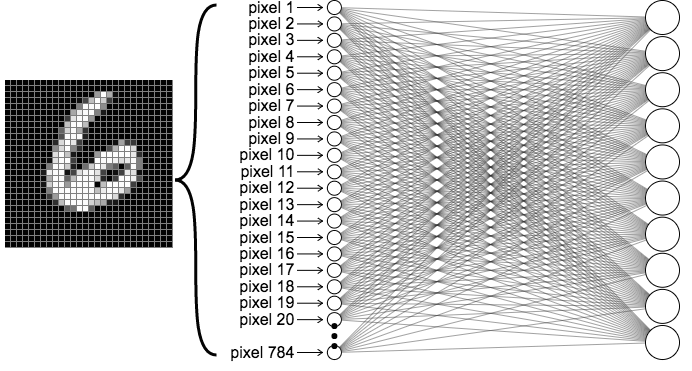
\includegraphics[width = 0.8 \textwidth]{media/mnist_1layer.png}
\end{center}

Das Programm erhält als Eingabe ein Bild. Im Beispiel ist das ein Graustufen-Bild mit $28\times28 =784$ Pixel. Nun soll der Computer entscheiden, um welche Zahl es sich dabei handelt.
Das Input-Bild kann als Vektor $\vec{v}$ mit 784 Komponenten gelesen werden, wobei z.B. in der 30. Komponente steht, wie dunkel der entsprechende Pixel (2. Pixel in der 2. Zeile) auf einer Skala von 0 bis 1 ist. Dieser Vektor wird dann mit einer $10\times784$-Matrix $M$ multipliziert und damit in einen Vektor $\vec{w} = M \cdot \vec{v}$ mit 10 Einträgen verwandelt. In diesem Vektor $\vec{w}$ steht dann, wie wahrscheinlich das Bild eine bestimmte Ziffer darstellt. So steht z.B. im 4. Eintrag von $\vec{w}$  die Wahrscheinlichkeit, dass es sich beim Bild um eine Vier handelt, im 10. Eintrag steht die Wahrscheinlichkeit für eine Null.
Die Frage ist nur noch: Wie lauten die 7840 Einträge der Matrix $M$? Die Kernidee des maschinellen Lernens ist, dass man den Computer diese Einträge selber lernen lässt! Dazu braucht es einiges an Mathematik. Mehr dazu im Schwerpunktfach AM oder im Ergänzungsfach I\dots

